\documentclass[12pt,a4paper]{scrartcl}
\usepackage[utf8]{inputenc}
\usepackage[english,russian]{babel}
\usepackage{indentfirst}
\usepackage{misccorr}
\usepackage{graphicx}
\usepackage{amsmath}
\usepackage{multirow}
\usepackage{pgfplots}
\usepackage[top=1cm, bottom=1cm, left=1cm, right=1cm]{geometry}
\pgfplotsset{compat=1.9}

\begin{document}
	\graphicspath{{C:/Users/Alex/OneDrive/Изображения/TexImgs}}
	
	\newcommand{\ms}{\mathstrut}
	\newcommand{\msp}{\hspace{0.5cm}}
	\newcommand{\al}{\alpha}
	\newcommand{\dg}{^\circ}
	\newcommand{\qd}[2]{^{\frac{#1}{#2}}}
	\newcommand{\qdm}[2]{^{-\frac{#1}{#2}}}
	\newcommand{\lm}[2]{\underset{#1 \rightarrow #2}{\lim}}
	\newcommand{\sfrac}[2]{\dfrac{\strut #1}{\strut #2}}
	\newcommand{\equal}[1]{\overset{(#1)}{=}}
	\newcommand{\linevdots}{\ \raisebox{-.08\height}{\vdots}\ }
	\newcommand{\linecvdots}{\ \raisebox{-.08\height}{\vdots}\hspace{-0.13cm}\raisebox{.15\height}{\cancel{\phantom{a}}\hspace{0.06cm}}}
	\newcommand{\combox}[1]{\ms \msp \msp \begin{minipage}{0.95\linewidth}
			#1
	\end{minipage}}
	
	\newtheorem{pr}{Задача}
	\newtheorem{ex}{Пример}
	\newtheorem{dfn}{Def}
	\newtheorem{theorem}{Th}
	
	\newenvironment{slv}{\ms \msp \textit{Решение:}}{}
	\newenvironment{proof}{\ms \msp \textit{Доказательство: }}{\hfill $\square$}
	
	\begin{titlepage}
		
		\vspace*{\fill}
		
		\begin{center}
			
\includegraphics[scale=0.8]{MIPT.png}
			\\[0.7cm]\Huge Московский Физико-Технический Институт\\(национальный исследовательский университет)
			\\[2cm]\LARGE Отчет по эксперименту
			\\[0.5cm]\noindent\rule{\textwidth}{1pt}
			\\\Huge\textbf{Исследование прецессии\\уравновешенного гироскопа}
			\\[-0.5cm]\noindent\rule{\textwidth}{1pt}
		\end{center}
		
		\begin{flushleft}
			\textit{Работа №1.2.5; дата: 15.11.21}\hfill\textit{Семестр: 1}
		\end{flushleft}
		
		\vspace*{\fill}
		
		\begin{flushleft}
			Выполнил: \hspace{\fill} Группа:
			\\Кошелев Александр \hspace{\fill} Б05-105
		\end{flushleft}
	\end{titlepage}
	
	%Страница 2
	
	\begin{flushleft}
		\footnotesize{Исследование прецессии уравновешенного гироскопа} \hspace{\fill} \footnotesize{2}
		\\[-0.3cm]\noindent\rule{\textwidth}{0.3pt}
	\end{flushleft}

	\section{Аннотация}
	
	В данной работе исследуется вынужденная прецессия гироскопа, устанавливается зависимость скорости вынужденной прецессии от величины момента сил, действующих на ось гироскопа, а также определяется скорость вращения ротора гироскопа и сравнивается со скоростью, рассчитанной по скорости прецессии.

	\textbf{Схема установки:}
	\begin{center}
		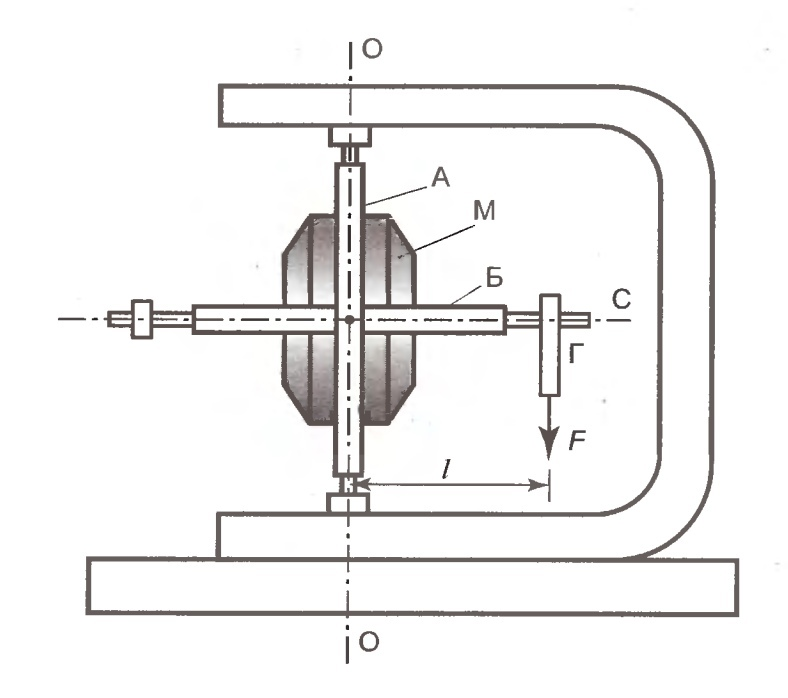
\includegraphics[scale=0.2]{PIC_1.jpg}
		\\\textbf{Рис. 1:} Схема установки
	\end{center}
	

	\textbf{В работе используются:} гироскоп в карданном подвесе, секундомер, набор грузов, отдельный ротор гироскопа, цилиндр известной массы и диаметра, крутильный маятник, штангенциркуль, линейка.
	 

	\section{Теоретические сведения}
	Запишем уравнение движения твёрдого тела:
	\begin{equation}
		\dot{\vec{P}} = \vec{F}
	\end{equation}
	
	Также запишем уравнение моментов:
	\begin{equation}
		\dot{\vec{L}} = \vec{M}
	\end{equation}

	Выразим момент импульса тела:
	\begin{equation}
		\vec{L} = \vec{i} I_x \omega_x +  \vec{j} I_y \omega_y +  \vec{k} I_z \omega_z
	\end{equation}

	Где $I_x, I_y, I_z $ -- главные оси инерции; $\omega_x, \omega_y, \omega_z$ -- компоненты вектора угловой скорости $ \vec{\omega} $.
	
	В силу (2), принимая во внимание $I_z \omega_z \gg I_x \omega_x, I_y \omega_y$:
	\begin{equation}
		\Delta \vec{L} = \int \vec{M} \cdot  dt
	\end{equation}

	%Страница 3
	
	\begin{flushleft}
		\footnotesize{Исследование прецессии уравновешенного гироскопа} \hspace{\fill} \footnotesize{3}
		\\[-0.3cm]\noindent\rule{\textwidth}{0.3pt}
	\end{flushleft}

	Если момент сил действует в течении малого времени, то гироскоп устойчив -- $|\Delta \vec{L}| \ll |\vec{L}|$ 
	
	\begin{equation}
		\vec{M} = [\vec{\Omega}, \vec{L}]
	\end{equation}
	
	\begin{equation}
		\dot{\vec{L}} = [\vec{\Omega}, \vec{L}] 
	\end{equation}
	
	Выразим $|\vec{\Omega}|$ -- скорость прецессии
	
	\begin{equation}
		\Omega = \frac{mgl}{I_z \omega_0}
	\end{equation}
	
	Где $m$ -- масса груза, $l$ -- расстояние от центра карданного подвеса до точки крепления груза.
	
	Момент инерции ротора $I_z$ можно определить через момент инерции цилиндра $I_c$, параметры \par которого можно измерить, и периоды их крутильных колебаний на проволоке:
	
	\begin{equation}
		I_z  = I_{c} \cdot \frac{T_0^2}{T_{c}^2}
	\end{equation}
	
	\section{Проведение эксперимента}
	\paragraph{Измерение скорости прецессии} \hfill
	\par Проведём измерения для грузов 9 различных масс, проведя по 2 измерения для каждой массы и занесём результаты в таблицу. Момент силы тяжести груза также подсчитаем, для нашей установки плечо силы тяжести $l = 11.91 \pm 0.05\,\text{см}$.
	
	\begin{center}
		\begin{tabular}{|c|c|c|c|c|c|c|}
			\hline
			№  & $T$, с & $\Omega$, с$^{-1}$ & $h_0$, см & $h_1$, см & $m$, г          & $M$, кг$\,\cdot\,$м$^2$/с$^2$\\ \hline
			1  & 178.98 $\pm$ 0.50 & 0.0351 $\pm$ 0.0001 & 11.7 & 10.5 & 56.2  $\pm$ 0.1 & 0.0656 $\pm$ 0.0001\\ \hline
			2  & 180.81 $\pm$ 0.50 & 0.0348 $\pm$ 0.0001 & 11.7 & 10.3 & 56.2  $\pm$ 0.1 & 0.0656 $\pm$ 0.0001\\ \hline
			3  & 135.83 $\pm$ 0.50 & 0.0463 $\pm$ 0.0002 & 11.7 & 10.5 & 74.4  $\pm$ 0.1 & 0.0869 $\pm$ 0.0001\\ \hline
			4  & 136.38 $\pm$ 0.50 & 0.0461 $\pm$ 0.0002 & 11.7 & 10.3 & 74.4  $\pm$ 0.1 & 0.0869 $\pm$ 0.0001\\ \hline
			5  & 110.47 $\pm$ 0.50 & 0.0569 $\pm$ 0.0003 & 11.7 & 11.0 & 91.5  $\pm$ 0.1 & 0.1068 $\pm$ 0.0001 \\ \hline
			6  & 110.46 $\pm$ 0.50 & 0.0569 $\pm$ 0.0003 & 11.7 & 10.8 & 91.5  $\pm$ 0.1 & 0.1068 $\pm$ 0.0001\\ \hline
			7  & 86.92  $\pm$ 0.50 & 0.0723 $\pm$ 0.0004 & 11.7 & 10.7 & 116.2 $\pm$ 0.1 & 0.1357 $\pm$ 0.0001\\ \hline
			8  & 86.74  $\pm$ 0.50 & 0.0724 $\pm$ 0.0004 & 11.7 & 11.0 & 116.2 $\pm$ 0.1 & 0.1357 $\pm$ 0.0001\\ \hline
			9  & 71.28  $\pm$ 0.50 & 0.0881 $\pm$ 0.0006 & 11.7 & 11.0 & 141.8 $\pm$ 0.1 & 0.1655 $\pm$ 0.0001\\ \hline
			10 & 71.49  $\pm$ 0.50 & 0.0879 $\pm$ 0.0006 & 11.7 & 11.2 & 141.8 $\pm$ 0.1 & 0.1655 $\pm$ 0.0001\\ \hline
			11 & 55.85  $\pm$ 0.50 & 0.1125 $\pm$ 0.0010 & 11.7 & 11.2 & 179.1 $\pm$ 0.1 & 0.2091 $\pm$ 0.0001\\ \hline
			12 & 56.67  $\pm$ 0.50 & 0.1109 $\pm$ 0.0010 & 11.7 & 11.3 & 179.1 $\pm$ 0.1 & 0.2091 $\pm$ 0.0001\\ \hline
			13 & 46.28  $\pm$ 0.50 & 0.1358 $\pm$ 0.0015 & 11.7 & 11.4 & 218.9 $\pm$ 0.1 & 0.2555 $\pm$ 0.0001\\ \hline
			14 & 26.31  $\pm$ 0.50 & 0.1359 $\pm$ 0.0015 & 11.7 & 11.4 & 218.9 $\pm$ 0.1 & 0.2555 $\pm$ 0.0001\\ \hline
			15 & 37.57  $\pm$ 0.50 & 0.1672 $\pm$ 0.0022 & 11.7 & 11.5 & 272.2 $\pm$ 0.1 & 0.3178 $\pm$ 0.0001\\ \hline
			16 & 37.23  $\pm$ 0.50 & 0.1688 $\pm$ 0.0023 & 11.7 & 11.4 & 272.2 $\pm$ 0.1 & 0.3178 $\pm$ 0.0001\\ \hline
			17 & 29.76  $\pm$ 0.50 & 0.2111 $\pm$ 0.0035 & 11.7 & 11.6 & 340.6 $\pm$ 0.1 & 0.3976 $\pm$ 0.0001\\ \hline
			18 & 29.74  $\pm$ 0.50 & 0.2113 $\pm$ 0.0036 & 11.7 & 11.7 & 340.6 $\pm$ 0.1 & 0.3976 $\pm$ 0.0001\\ \hline
		\end{tabular}
		\\\textbf{Табл. 1: } Измерение скорости прецессии
	\end{center}
	
	На основе этих данных построим график и определим коэффициент пропорциональности $\lambda$ между моментом силы тяжести $M$, действующей на груз, и угловой скоростью прецессии $\Omega$.
	
	\newpage
	%Страница 4
	
	\begin{flushleft}
		\footnotesize{Исследование прецессии уравновешенного гироскопа} \hspace{\fill} \footnotesize{4}
		\\[-0.3cm]\noindent\rule{\textwidth}{0.3pt}
	\end{flushleft}

	\begin{center}
		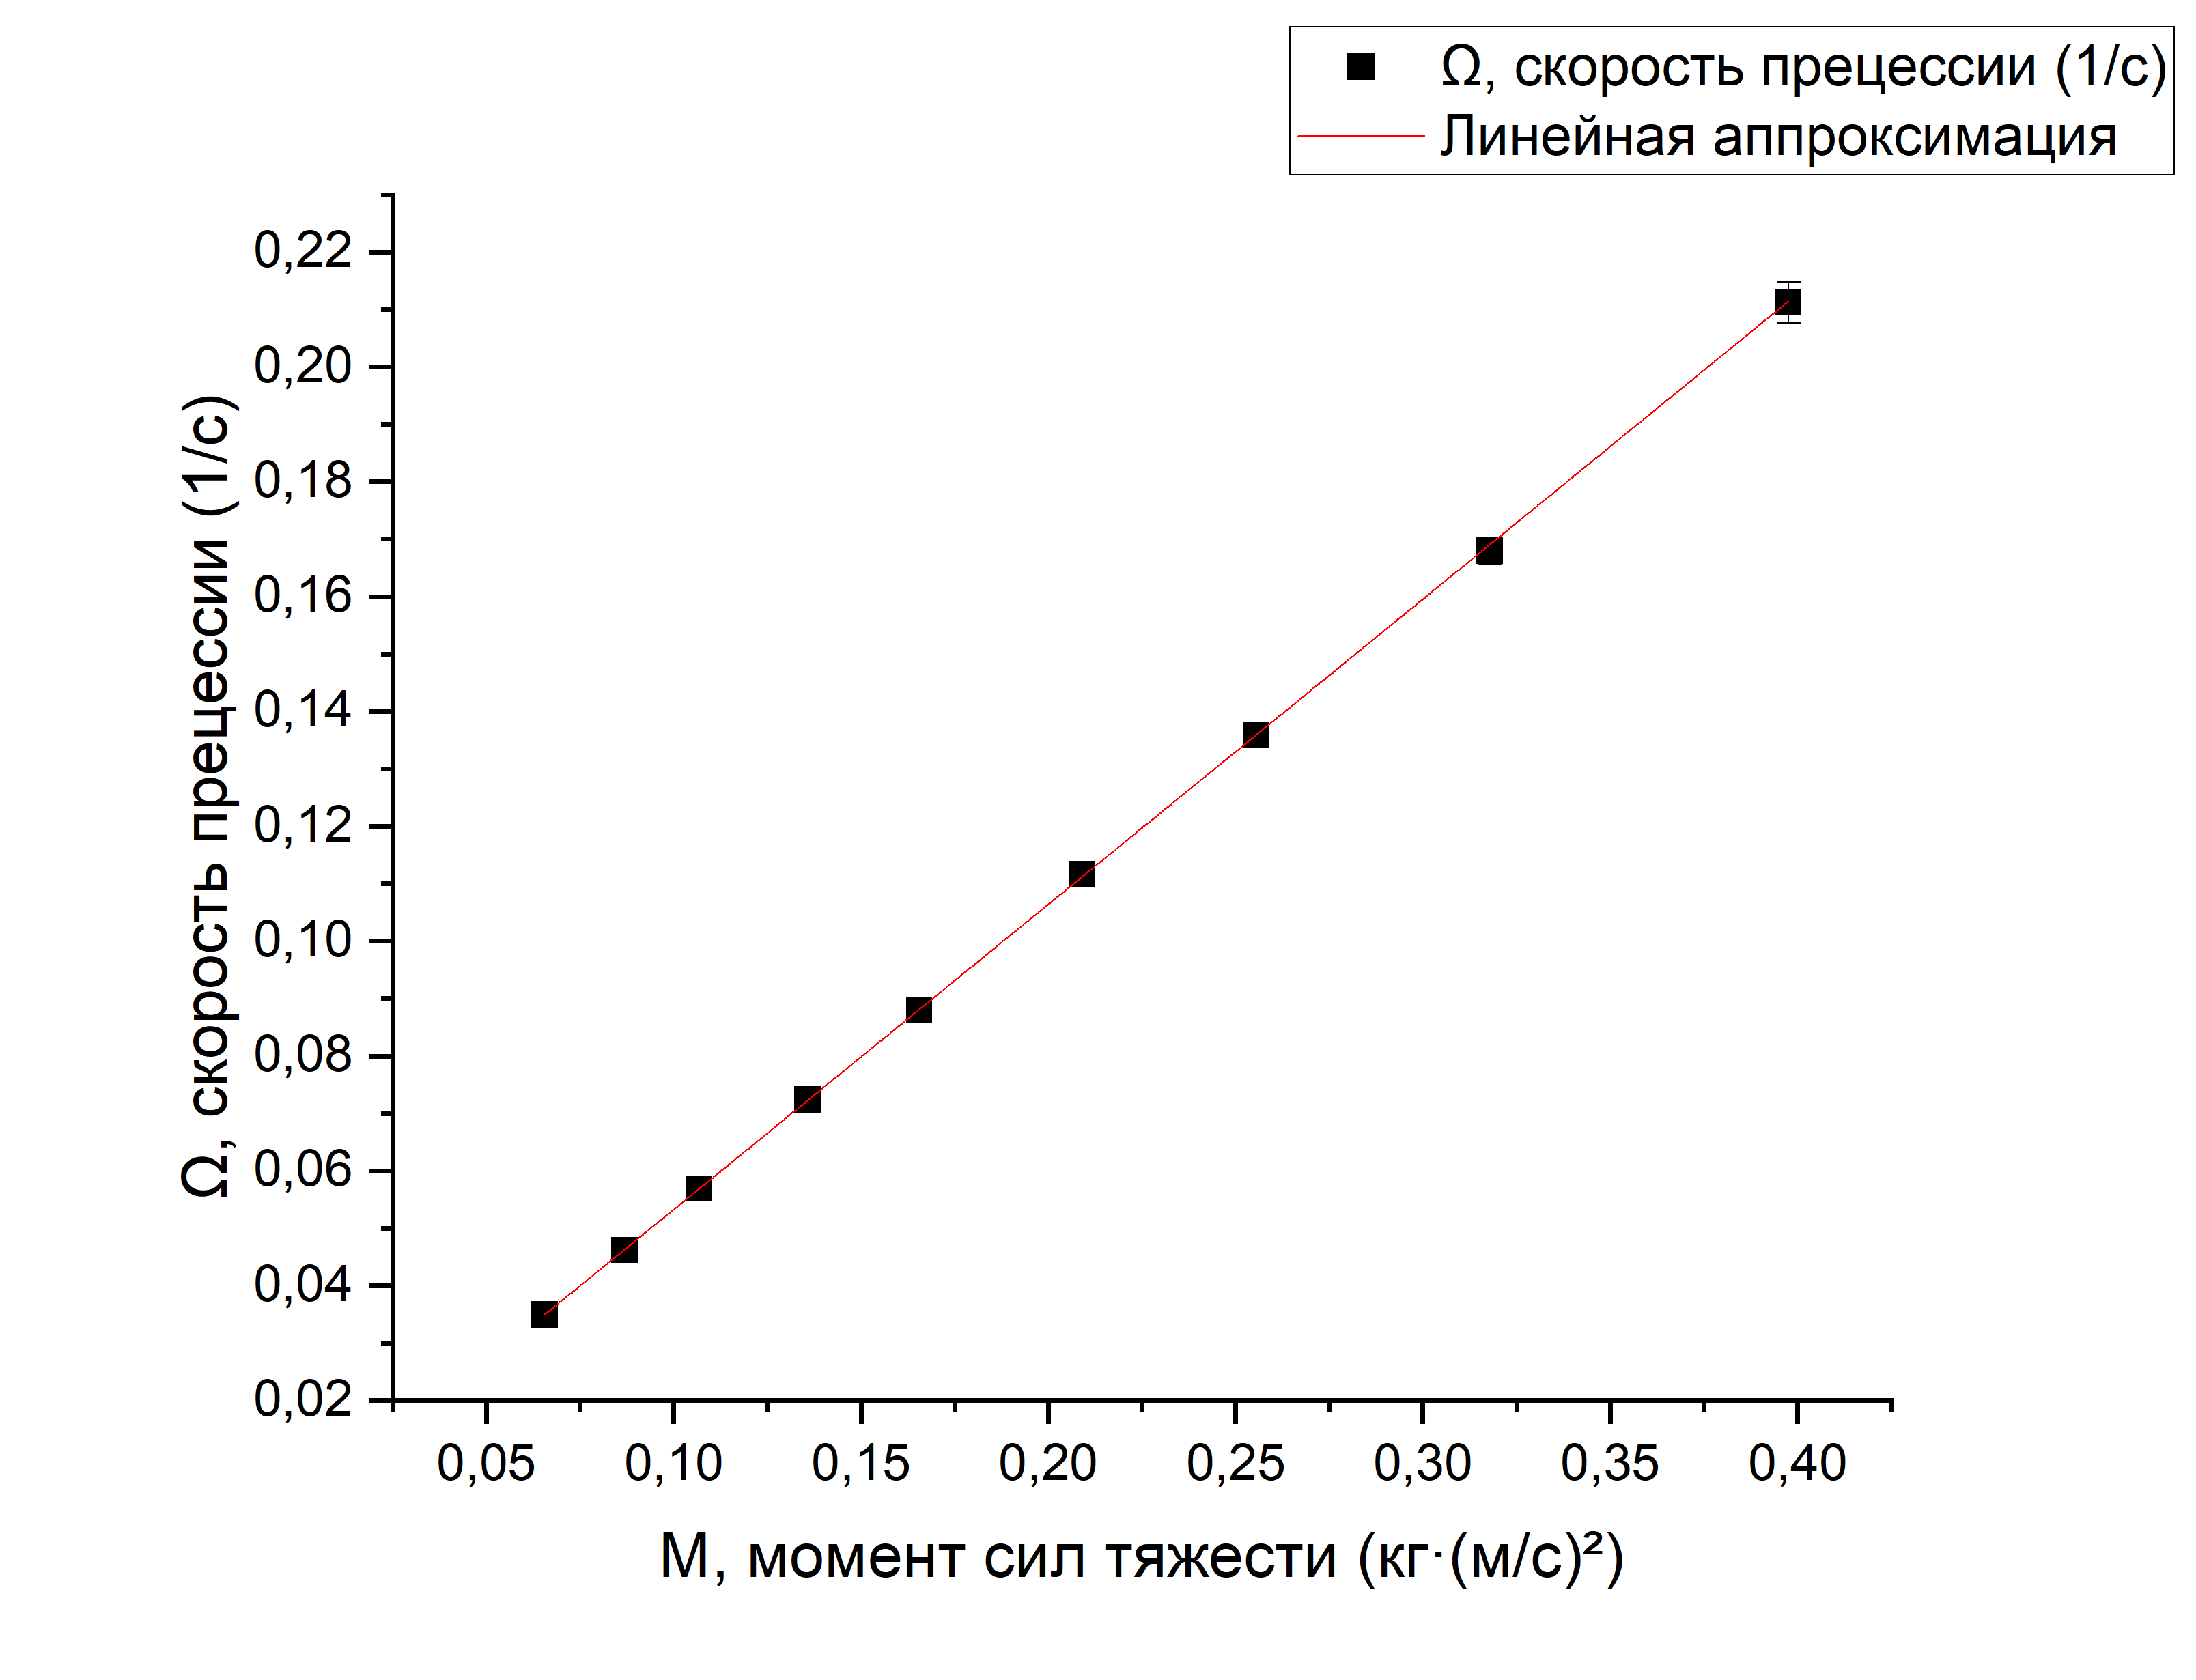
\includegraphics[scale=0.5]{PIC_2.png}
		\\\textbf{Рис. 2: } График зависимости $\Omega(M)$
	\end{center}

	Путем линейной аппроксимации получаем:
	\begin{equation}
		\sfrac{1}{I_z\omega_0} = \lambda = 0.532 \pm 0.001\ \sfrac{\text{кг}\cdot\text{с}}{\text{м}^2}
	\end{equation}
	
	\paragraph{Измерение момента инерции ротора} \hfill
	\par Вначале измерим параметры калибровочного цилиндра, представим таблично:
	
	\begin{center}
		\begin{tabular}{|c|c|c|}
			\hline
			$m$, кг & $d$, м & $I_c$, кг$\,\cdot\,$м$^2$ \\\hline
			1.6178 $\pm$ 0.0001 & 0.0781 $\pm$ 0.0001 & (1.233 $\pm$ 0.006) $\cdot 10^{-3}$ \\\hline
		\end{tabular}
		\\\textbf{Табл. 2: } Параметры калибровочного цилиндра
	\end{center}

	Теперь определим периоды крутильных колебаний калибровочного цилиндра и ротора на проволоке:

	\begin{center}
		\begin{tabular}{|c|c|c|c|}
			\hline
			$10 \cdot T_c$, c & $10 \cdot T_0$, c & $T_c$, c & $T_0$, c \\ \hline
			40.35 $\pm$ 0.5 & 31.97 $\pm$ 0.5 & \multirow{5}{*}{4.04 $\pm$ 0.06} & \multirow{5}{*}{3.26 $\pm$ 0.06}   \\ \cline{1-2}
			40.22 $\pm$ 0.5 & 32.09 $\pm$ 0.5 &&    \\ \cline{1-2}
			40.50 $\pm$ 0.5 & 32.10 $\pm$ 0.5 &&    \\ \cline{1-2}
			40.41 $\pm$ 0.5 & 32.10 $\pm$ 0.5 &&    \\ \cline{1-2}
			40.53 $\pm$ 0.5 & 32.05 $\pm$ 0.5 &&    \\ \hline
		\end{tabular}
		\\\textbf{Табл. 3: } Периоды крутильных колебаний
	\end{center}

	Воспользуемся соотношением (8) для определения момента инерции ротора:
	$$I_z = (8.029 \pm 0.096) \cdot 10^{-4}\ \text{кг} \cdot \text{м}^2$$
	
	\newpage
	%Страница 5
	
	\begin{flushleft}
		\footnotesize{Исследование прецессии уравновешенного гироскопа} \hspace{\fill} \footnotesize{5}
		\\[-0.3cm]\noindent\rule{\textwidth}{0.3pt}
	\end{flushleft}
	
	Таким образом, исходя из $I_z$ и коэффициента $\lambda$, получаем угловую скорость и частоту вращения ротора:
	\begin{equation*}
		\omega_0 = 2340 \pm 30\, \text{с}^{-1}
	\end{equation*}

	\begin{equation*}
		\nu_0 = 372 \pm 5\, \text{Гц}
	\end{equation*}
	
	\paragraph{Определение частоты вращения ротора с помощью осциллографа} \hfill
	
	\par Ротор гироскопа всегда немного намагничен, поэтому он наводит переменную ЭДС индукции в контрольной обмотке. Частота этой ЭДС совпадает с частотой вращения ротора, поэтому так можно получить контрольное значение по фигуре Лиссажу.
	
	\par Путем приближения к частоте гироскопа обнаруживаем, что наблюдаем эллиптическую фигуру Лиссажу на частоте $\nu_1 \approx 370 \pm 1\, \text{Гц}$.
	
	\paragraph{Определение момента сил трения} \hfill
	
	\par Известно, что в осях гироскопа есть трение. При наблюдаемой прецессии сила трения создает момент, провоцирующий прецессию-опускание оси гироскопа. Обозначим угловую скорость опускания как $\Omega_f$. При этом угол $\varphi_f$ опускания в приближении малости угла можно записать как:
	
	$$\varphi_f = \sfrac{h_0 - h_1}{l}$$
	
	Тогда угловая скорость опускания:
	
	$$\Omega_f = \sfrac{\varphi_f}{T} = \sfrac{h_0 - h_1}{Tl}$$
	
	Согласно формуле (5) запишем момент инерции силы трения:
	
	$$M_f = \Omega_f I_z \omega_0$$
	
	Тогда рассчитаем значения момента по данным из Табл. 1 и усредним их:
	
	$$M_f \approx 1\,\text{мН} \cdot\text{м}$$

	\section{Выводы}
	В ходе эксперимента были получены разными способами значения частоты вращения ротора гироскопа:
	\begin{equation*}
		\nu_0 = 372 \pm 5\, \text{Гц}
	\end{equation*}
	\begin{equation*}
		\nu_1 = 370 \pm 1\, \text{Гц}
	\end{equation*}
	
	Полученные значения лежат в пределах одной величины погрешности друг от друга, что говорит о справедливости предположений, сделанных в теоретических выкладках. При этом относительные погрешности оказались довольно невелики $\varepsilon \approx 1\%$.
	
	Также в работе установлен приблизительный момент сил трения в оси гироскопа:
	
	$$M_f \approx 1\,\text{мН} \cdot\text{м}$$
	
	Значение приводится лишь приближенно, поскольку для точных оценок необходимо точнее измерять углы отклонения гироскопа, например, при помощи округлой градусной шкалы рядом с осью.	
\end{document}